\begin{figure*}[t]
\begin{center}
\bgroup 
 \def\arraystretch{0.2} 
 \setlength\tabcolsep{0.2pt}
\begin{tabular}{ccccc}
Input & Ground truth & L1 & cGAN & L1 + cGAN \\ 
%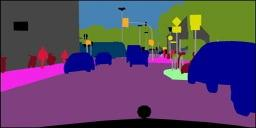
\includegraphics[width=0.2\linewidth]{figs/cityscapes_loss_variations_latex/input_407.jpg} &
%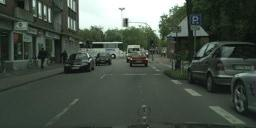
\includegraphics[width=0.2\linewidth]{figs/cityscapes_loss_variations_latex/gt_407.jpg} &
%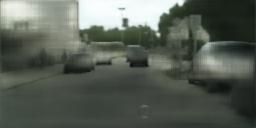
\includegraphics[width=0.2\linewidth]{figs/cityscapes_loss_variations_latex/L1_407.jpg} &
%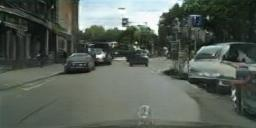
\includegraphics[width=0.2\linewidth]{figs/cityscapes_loss_variations_latex/cGAN_407.jpg} &
%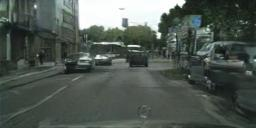
\includegraphics[width=0.2\linewidth]{figs/cityscapes_loss_variations_latex/L1cGAN_407.jpg} \\ 
%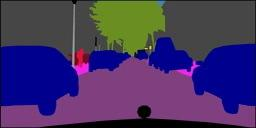
\includegraphics[width=0.2\linewidth]{figs/cityscapes_loss_variations_latex/input_426.jpg} &
%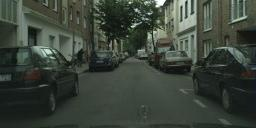
\includegraphics[width=0.2\linewidth]{figs/cityscapes_loss_variations_latex/gt_426.jpg} &
%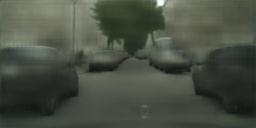
\includegraphics[width=0.2\linewidth]{figs/cityscapes_loss_variations_latex/L1_426.jpg} &
%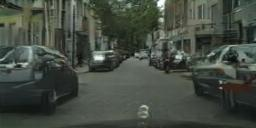
\includegraphics[width=0.2\linewidth]{figs/cityscapes_loss_variations_latex/cGAN_426.jpg} &
%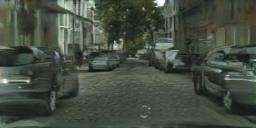
\includegraphics[width=0.2\linewidth]{figs/cityscapes_loss_variations_latex/L1cGAN_426.jpg} \\
%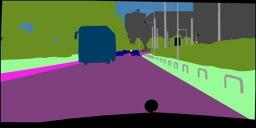
\includegraphics[width=0.2\linewidth]{figs/cityscapes_loss_variations_latex/input_15.jpg} &
%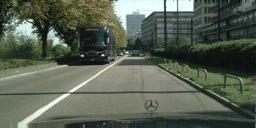
\includegraphics[width=0.2\linewidth]{figs/cityscapes_loss_variations_latex/gt_15.jpg} &
%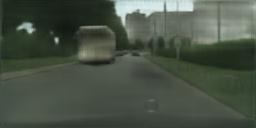
\includegraphics[width=0.2\linewidth]{figs/cityscapes_loss_variations_latex/L1_15.jpg} &
%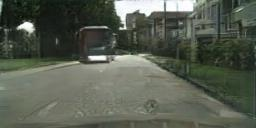
\includegraphics[width=0.2\linewidth]{figs/cityscapes_loss_variations_latex/cGAN_15.jpg} &
%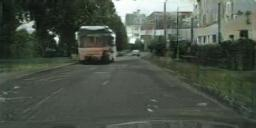
\includegraphics[width=0.2\linewidth]{figs/cityscapes_loss_variations_latex/L1cGAN_15.jpg} \\ 
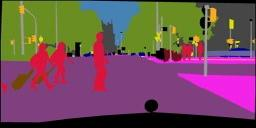
\includegraphics[width=0.2\linewidth]{figs/cityscapes_loss_variations_latex/input_116.jpg} &
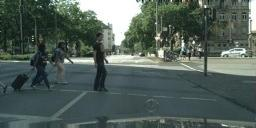
\includegraphics[width=0.2\linewidth]{figs/cityscapes_loss_variations_latex/gt_116.jpg} &
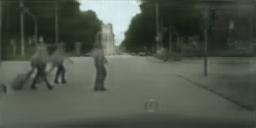
\includegraphics[width=0.2\linewidth]{figs/cityscapes_loss_variations_latex/L1_116.jpg} &
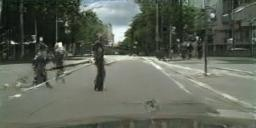
\includegraphics[width=0.2\linewidth]{figs/cityscapes_loss_variations_latex/cGAN_116.jpg} &
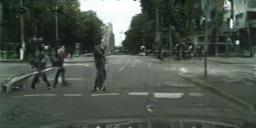
\includegraphics[width=0.2\linewidth]{figs/cityscapes_loss_variations_latex/L1cGAN_116.jpg} \\ 
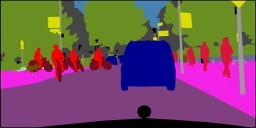
\includegraphics[width=0.2\linewidth]{figs/cityscapes_loss_variations_latex/input_382.jpg} &
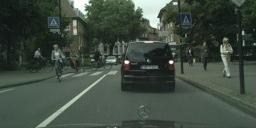
\includegraphics[width=0.2\linewidth]{figs/cityscapes_loss_variations_latex/gt_382.jpg} &
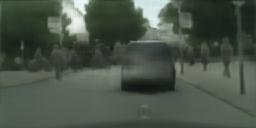
\includegraphics[width=0.2\linewidth]{figs/cityscapes_loss_variations_latex/L1_382.jpg} &
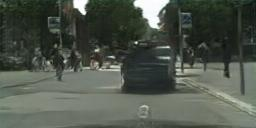
\includegraphics[width=0.2\linewidth]{figs/cityscapes_loss_variations_latex/cGAN_382.jpg} &
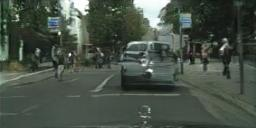
\includegraphics[width=0.2\linewidth]{figs/cityscapes_loss_variations_latex/L1cGAN_382.jpg} \\

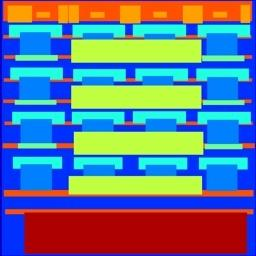
\includegraphics[width=0.2\linewidth]{figs/facades2_loss_variations_latex/input_46.jpg} &
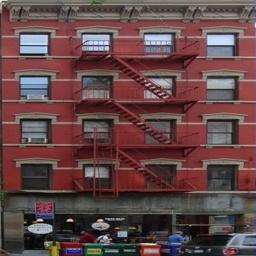
\includegraphics[width=0.2\linewidth]{figs/facades2_loss_variations_latex/gt_46.jpg} &
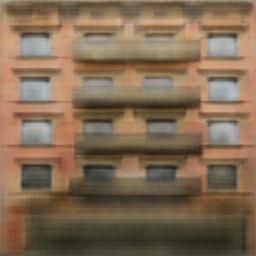
\includegraphics[width=0.2\linewidth]{figs/facades2_loss_variations_latex/L1_46.jpg} &
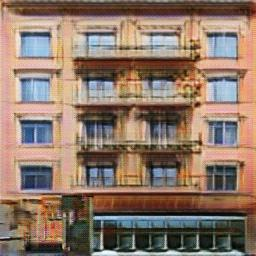
\includegraphics[width=0.2\linewidth]{figs/facades2_loss_variations_latex/cGAN_46.jpg} &
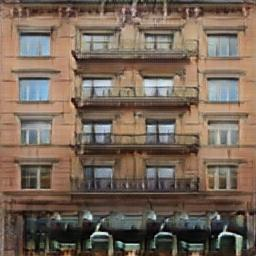
\includegraphics[width=0.2\linewidth]{figs/facades2_loss_variations_latex/L1cGAN_46.jpg} \\ 

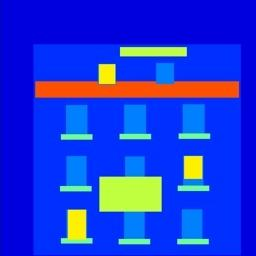
\includegraphics[width=0.2\linewidth]{figs/facades2_loss_variations_latex/input_60.jpg} &
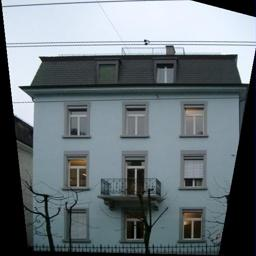
\includegraphics[width=0.2\linewidth]{figs/facades2_loss_variations_latex/gt_60.jpg} &
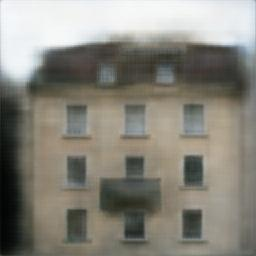
\includegraphics[width=0.2\linewidth]{figs/facades2_loss_variations_latex/L1_60.jpg} &
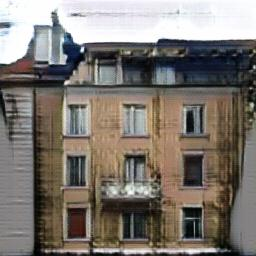
\includegraphics[width=0.2\linewidth]{figs/facades2_loss_variations_latex/cGAN_60.jpg} &
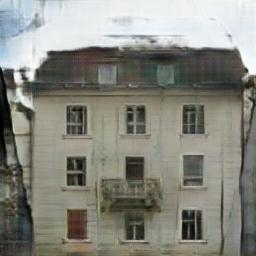
\includegraphics[width=0.2\linewidth]{figs/facades2_loss_variations_latex/L1cGAN_60.jpg}

\end{tabular} \egroup 
\end{center}
\vspace{-0.2in}
\caption{Different losses induce different quality of results. Each column shows results trained under a different loss. Please see \texttt{https://phillipi.github.io/pix2pix/} for additional examples.}
\label{cityscapes_loss_variations_qualitative}
\vspace{-0.2in}
\end{figure*}